\pdfoutput=1
% IEEE S&P 2027 (Cycle 2) anonymous submission.
% Double-blind: no author names, affiliations, ORCID, acknowledgments, or identifying links.
\documentclass[conference,compsoc]{IEEEtran}
\IEEEoverridecommandlockouts

\usepackage[T1]{fontenc}
\usepackage[utf8]{inputenc}
\usepackage[nocompress]{cite}
\usepackage{amsmath,amssymb}
\usepackage{graphicx}
\usepackage{booktabs}
\usepackage{array}
\usepackage{tabularx}
\usepackage{multirow}
\usepackage{listings}
\usepackage{xcolor}
\usepackage{balance}
\usepackage{url}
\usepackage[hidelinks]{hyperref}
\hypersetup{pdfauthor={Anonymous},pdftitle={Sealed Decoding: Encrypting PII Inside the LLM Generate Loop}}

\graphicspath{{figures/}}
\newcommand{\code}[1]{\texttt{#1}}
\newcommand{\tok}[3]{\texttt{\textless{}PII:#1:\allowbreak#2\ldots#3\textgreater{}}}
\newcolumntype{L}{>{\raggedright\arraybackslash}X}
\newcolumntype{P}[1]{>{\raggedright\arraybackslash}p{#1}}
\newcommand{\margonMs}{18.3}
\newcommand{\margonRange}{18.0--23.8}
\newcommand{\msealUs}{22}
\newcommand{\mopenUs}{5}
\newcommand{\mdetectUs}{16}
\newcommand{\mssnTokLen}{121}
\newcommand{\memailTokLen}{147}
\newcommand{\mcliMs}{83.7}
\newcommand{\mcliRss}{270}
\newcommand{\mrawS}{1.99}
\newcommand{\mrawRange}{1.95--2.13}
\newcommand{\msealedS}{1.91}
\newcommand{\msealedRange}{1.89--2.42}
\newcommand{\mhookMs}{2.48}
\newcommand{\mhookRange}{2.16--2.88}
\newcommand{\mttfbRaw}{210}
\newcommand{\mttfbSealed}{209}
\newcommand{\mgenRss}{2108}
\newcommand{\mgenLoad}{1.59}
\newcommand{\mgenRuns}{5}
\newcommand{\mgenPrompt}{161}
\newcommand{\mgenChunks}{44}
\newcommand{\menvPy}{3.13.5}
\newcommand{\menvTorch}{2.14.1+cpu}
\newcommand{\menvTf}{5.20.2}
\newcommand{\menvCrypto}{50.0.2}
\newcommand{\menvArgon}{25.1.0}
\newcommand{\menvCpus}{8}

\makeatletter\newcommand{\inputrows}[1]{\@@input #1 }\makeatother

\lstset{basicstyle=\ttfamily\scriptsize, columns=fullflexible, keepspaces=true,
  showstringspaces=false, frame=tb, framerule=0.4pt, aboveskip=4pt, belowskip=2pt,
  literate={↩}{{$\hookleftarrow$}}1, upquote=true}

\renewcommand{\topfraction}{0.9}
\renewcommand{\dbltopfraction}{0.9}
\renewcommand{\textfraction}{0.1}
\renewcommand{\floatpagefraction}{0.85}
\renewcommand{\dblfloatpagefraction}{0.85}
\setcounter{topnumber}{3}
\setcounter{dbltopnumber}{2}

\begin{document}

\title{Sealed Decoding: Encrypting PII Inside the\\LLM Generate Loop}

\author{\IEEEauthorblockN{Anonymous Submission}
\IEEEauthorblockA{Paper under double-blind review}}

\maketitle

\begin{abstract}
Language models that answer over private documents copy personal data into their output. Most deployments stream that output token by token, so a filter that runs on the finished answer acts after the client already has the data, and a filter that runs before the model removes the data for everyone, including readers who are entitled to it. We describe Sealed Decoding, a serving pattern that encrypts personally identifiable information (PII) inside the generate loop. A streaming hook holds back any suffix that could still grow into a PII span and replaces each completed span with an AES-256-GCM ciphertext under a per-model data key, which is wrapped by an Argon2id key derived from an operator password. Only ciphertexts issued by the current request that authenticate under the live key may leave the server; model-written look-alikes are stripped, and PII absent from the supplied context is not sealed. Password rotation rewraps the data key without touching weights or stored ciphertexts. The open-source implementation passes 62 automated tests. On Qwen3-0.6B on an 8-vCPU CPU host it seals an email address and a Social Security number while streaming, decrypts both with the right password, and fails closed with a wrong one (7/7 checks in three runs). The sealing hook costs about \mhookMs\,ms of CPU per request against roughly \msealedS\,s of generation. We show four synthetic user prompts end to end, including two injection attempts. We have not measured leak rates, detector recall, or task utility on a benchmark; that plan is stated and labeled as proposed.
\end{abstract}

\begin{IEEEkeywords}
large language models, personally identifiable information, privacy, authenticated encryption, AES-GCM, Argon2id, streaming inference, guardrails, prompt injection
\end{IEEEkeywords}

%=====================================================================
\section{Introduction}
\label{sec:intro}

A retrieval-augmented assistant receives a question and a patient note. The note contains an email address and a Social Security number (SSN). The answer repeats both, and the serving stack streams it to the browser as it is generated. A post-hoc redactor sees the complete answer only after the last token. By then the browser has the SSN.

We call the interval between a token being generated and the full answer reaching a filter the \emph{streaming leak window}. Ram~\cite{ram2025constrained} names the same gap and closes it by masking logits so that PII tokens are never produced. That works, but it destroys the value, and a clinician, fraud analyst, or lawyer often needs the exact identifier. Pre-model de-identification, as in PrivateGPT Headless~\cite{privategpt}, keeps the value away from the model but re-inserts it in plaintext afterwards, so the final stream still carries it.

We take a different position. The model is untrusted. So are the network, logs, caches, and downstream tools. The only party that should see a PII value in clear is the holder of a specific key. Under that position the right primitive is not deletion but authenticated encryption applied at token granularity, before any byte is flushed.

The idea is simple; the details are not. A streaming sealer must decide when a partial span is safe to emit. It must stop the model from writing text that looks like a ciphertext and would later be trusted. It must decide whether to seal a value the model invented. And it must let operators change passwords without re-encrypting stored outputs. This paper is about those details, and about what the system actually does when a user types a prompt.

\textbf{Contributions.}
\begin{enumerate}
  \item \textbf{Sealed Decoding}: a streaming hook, \code{EncryptedGenerator.on\_token}, that holds back partial PII and emits AES-256-GCM ciphertext in its place, so plaintext PII from the model is never written to the client stream (Section~\ref{sec:generator}).
  \item \textbf{Issued-only seals}: a per-request seal registry. A token-shaped string reaches the client only if this request created it and it authenticates under the live key (Section~\ref{sec:registry}).
  \item \textbf{Grounded sealing}: when the model is told not to answer from memory, only PII present in the supplied content or user messages is sealed; invented values are replaced or the request is refused (Section~\ref{sec:grounded}).
  \item \textbf{A key hierarchy for distribution}: Argon2id derives a key-encryption key that wraps a random data key; the wrapped key ships in a public header beside the weights, and rotation rewraps the same data key (Sections~\ref{sec:keyring}, \ref{sec:rotation}).
  \item \textbf{Measured, reproducible checks}: an open implementation with a Hugging Face backend for Qwen3, a breakdown of its 62 tests, real-model runs with wall times, per-operation costs, a token-level trace of one request, and four user prompts captured from the command line (Section~\ref{sec:validation}).
\end{enumerate}

%=====================================================================
\section{Background}
\label{sec:background}

\subsection{Autoregressive generation and streaming}

A decoder-only Transformer~\cite{vaswani2017attention} factorizes an output sequence as
\begin{equation}
  p(y \mid x) = \prod_{t=1}^{T} p(y_t \mid y_{<t}, x).
  \label{eq:ar}
\end{equation}
Serving stacks sample $y_t$, detokenize it, and usually flush the text to the client at once. The unit of exposure is a token or a small chunk, not an answer. A defense that promises ``no plaintext PII reaches the client'' has to act before each flush.

Tokens do not align with PII spans. An email address may arrive as eight or more sub-word pieces, and a detector cannot decide that \code{jsmith} belongs to an email until it sees \code{@} and a domain. Any token-level defense must buffer.

\subsection{How models leak PII}

Two sources matter. The first is memorized training data: Carlini et al.~\cite{carlini2021extracting} extracted verbatim training sequences, including contact details, from GPT-2 with query access only, and Lukas et al.~\cite{lukas2023analyzing} found that sentence-level differential privacy reduces but does not remove PII leakage from fine-tuned models. The second source is the context window. In retrieval and agent settings the model is handed documents that contain PII and asked about them; copying is the intended behavior. An inference-time guard can control this second source, and it is our focus.

\subsection{Where a guard can sit}

Table~\ref{tab:placement} compares the places a PII guard can run.

\begin{table}[!t]
\caption{Placement of a PII Guard and Its Consequences}
\label{tab:placement}
\centering
\footnotesize
\begin{tabularx}{\columnwidth}{@{}P{0.24\columnwidth}P{0.14\columnwidth}LL@{}}
\toprule
Placement & Acts on & Streaming leak window & Value for an authorized reader \\
\midrule
Pre-model de-identification & Prompt & Closed for the model; reopened at re-identification & Yes, via a side mapping, in plaintext \\
Post-hoc redaction & Finished answer & Open if streamed & No \\
Constrained decoding & Each step & Closed & No; never generated \\
\textbf{Sealed Decoding} & Each flushed chunk & Closed & Yes, with the key; ciphertext elsewhere \\
\bottomrule
\end{tabularx}
\end{table}

%=====================================================================
\section{Related Work}
\label{sec:related}

\textit{PII detectors and anonymizers.} Presidio~\cite{presidio} combines pattern recognizers, checksums, and NER models to find PII, then redacts, masks, hashes, or encrypts it. It operates on a complete string. Our detector is a much smaller pattern set and we claim no better recall. What we change is where detection runs (inside the stream, with hold-back) and what replaces a span (authenticated ciphertext bound to a tenant and entity type). A stronger detector could sit behind our hook without changing the rest of the design.

\textit{De-identification with re-identification.} PrivateGPT Headless~\cite{privategpt} replaces entities in the prompt with markers, sends the redacted prompt to a hosted model, and swaps the originals back into the response. This protects data from the model provider but not the response path. Sealed Decoding protects the response path. The two compose: de-identify before a hosted model, seal on the way out.

\textit{Programmable rails.} NeMo Guardrails~\cite{rebedea2023nemo} specifies which topics and dialogue paths a bot may follow, with input and output rails that call checks. Rails decide whether a turn may proceed; they do not say how a value inside an allowed answer is protected. Our injection scan is a crude rail, and sealing can run underneath an existing one.

\textit{Constrained decoding for privacy.} Ram~\cite{ram2025constrained} keeps a rolling window of generated text, matches regular expressions for structured PII, and masks logits that would extend a match. It targets the same streaming window and shares our regex-limited detector and its evasion risks. The outcomes differ: logit masking guarantees the value is absent; sealing guarantees it is present only as ciphertext. Logit masking also needs the sampler, while sealing needs only the text stream, so it also works with hosted APIs that expose no logits.

\textit{Deployed guardrail studies.} Asthana et al.~\cite{asthana2025deploying} report two deployments of a privacy guard with per-type detection F1 and measured detection latency. They do not address reversible protection. Their numbers are a reference point for the detector half of our system, which we have not yet measured.

%=====================================================================
\section{Method}
\label{sec:method}

\begin{figure*}[!t]
  \centering
  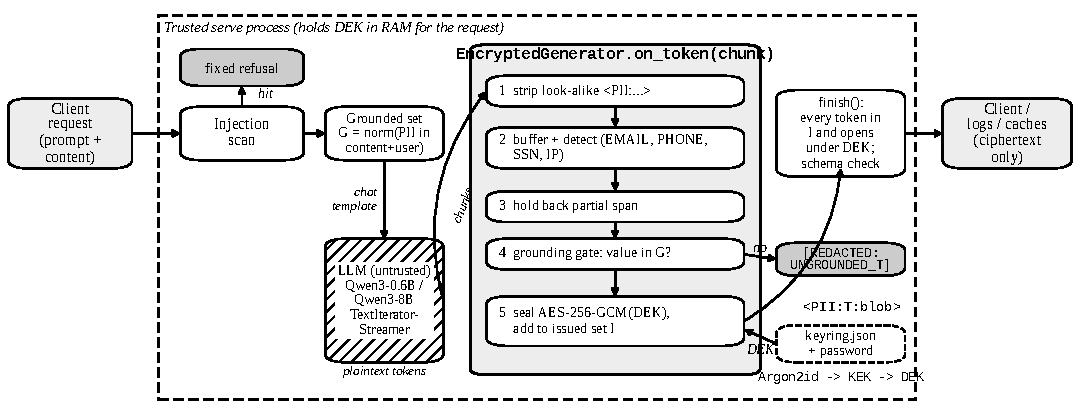
\includegraphics[width=\textwidth]{fig_pipeline.pdf}
  \caption{Serve path. The model and everything to the right of the serve process are untrusted. The serve process holds the data key (DEK) in memory for the request. A hit in the injection scan returns a fixed refusal without calling the model. Inside \code{on\_token}, each streamed chunk is (1) stripped of look-alike \code{<PII:\ldots>} text, (2) buffered and scanned, (3) held back while a span may still grow, (4) checked against the grounded set $G$, and (5) sealed and recorded in the issued set $I$. \code{finish()} re-verifies every token before the JSON response leaves.}
  \label{fig:pipeline}
\end{figure*}

Fig.~\ref{fig:pipeline} shows the request path. A request first passes an injection scan. Otherwise the model's token stream runs through the sealing hook, and the final output is re-verified before it leaves the server.

\subsection{Keyring}
\label{sec:keyring}

\begin{figure}[!t]
  \centering
  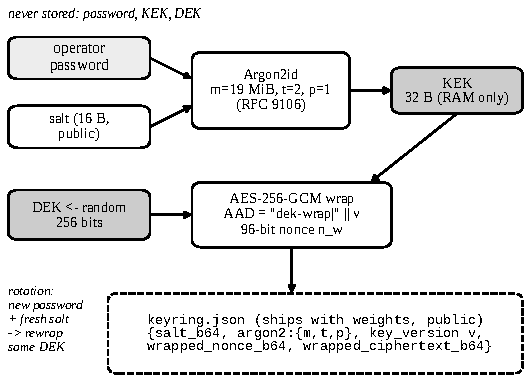
\includegraphics[width=\columnwidth]{fig_keyring.pdf}
  \caption{Key hierarchy. The password, KEK, and DEK are never written to disk. \code{keyring.json} is public and ships with the weights. Rotation derives a new KEK under a fresh salt and rewraps the same DEK, so earlier seals still open.}
  \label{fig:keyring}
\end{figure}

A model package carries a public header, \code{keyring.json} (Fig.~\ref{fig:keyring}). It holds a 16-byte random salt, the Argon2id parameters, a key version $v$, and the data key wrapped under a key-encryption key:
\begin{align}
  \mathrm{KEK} &= \mathrm{Argon2id}(\text{pw}, \text{salt};\ m{=}19\,\text{MiB}, t{=}2, p{=}1), \label{eq:kek}\\
  \mathrm{DEK} &\xleftarrow{\$} \{0,1\}^{256}, \label{eq:dek}\\
  w &= \mathrm{GCM}_{\mathrm{KEK}}\big(n_w, \mathrm{DEK};\ \texttt{"dek-wrap|"}\,\|\,v\big). \label{eq:wrap}
\end{align}
Argon2id follows RFC~9106~\cite{rfc9106} and GCM follows NIST SP~800-38D~\cite{nist80038d}. At serve time the operator supplies the password; the server derives the KEK, unwraps the DEK, and keeps it in process memory. A wrong password fails GCM authentication during unwrap, and no sealed session starts. The password never enters the prompt, the weights, or the header. The salt is public by design; it stops precomputation across packages.

\subsection{EncryptedGenerator: sealing inside the loop}
\label{sec:generator}

The serve path wraps the model's text iterator:
\begin{lstlisting}[language=Python]
gen = EncryptedGenerator(keys, tenant=tenant,
                         grounded_pii=grounded)
for chunk in model_stream:
    out = gen.on_token(chunk)
    if out:
        client.write(out)
client.write(gen.finish())
\end{lstlisting}
Each call to \code{on\_token} does four things.

\emph{Strip look-alikes.} Any substring matching \lstinline!<\s*PII\s*:! in model output becomes \code{[REDACTED:UNVERIFIED\_TOKEN]}, and its body is dropped up to the closing \code{>}. A tail such as \code{<P} that could still become \code{<PII:} is held until the next chunk resolves it.

\emph{Buffer and detect.} Sanitized text is appended to a buffer and the detector runs over it. It recognizes four structured types with regular expressions: \code{EMAIL}, \code{PHONE}, \code{SSN}, and \code{IP}.

\emph{Hold back.} The hook flushes only the longest prefix that cannot become part of a future span. It always holds the trailing word, since \code{jsmith} may become \code{jsmith@example.com}, and it holds trailing runs of digits and phone punctuation.

\emph{Seal.} A completed span becomes \code{<PII:TYPE:blob>}, where \code{blob} is base64url of \code{\{v, n, c, t\}} and
\begin{equation}
  c = \mathrm{GCM}_{\mathrm{DEK}}\big(n, \text{value};\ \text{tenant}\,|\,\text{TYPE}\,|\,v\big)
  \label{eq:seal}
\end{equation}
with a fresh 96-bit random nonce $n$. The token joins the request's issued set $I$. Random nonces mean the same value sealed twice gives two different tokens, so an observer cannot link two mentions of one SSN. Type and length stay visible (Section~\ref{sec:threat}). Fig.~\ref{fig:token} shows a real token from the healthcare run of Section~\ref{sec:userio}.

\begin{figure}[!t]
\lstinputlisting{generated/token.txt}
\caption{A real sealed SSN token from the healthcare prompt (Table~\ref{tab:userio}), copied from \code{paper/ieee/artifacts/examples/healthcare.json}. $\hookleftarrow$ marks a line wrap added for the column; no characters were removed. Field \code{n} is the GCM nonce, \code{c} the ciphertext plus tag.}
\label{fig:token}
\end{figure}

\subsection{Seal registry and verification}
\label{sec:registry}

\begin{figure}[!t]
  \centering
  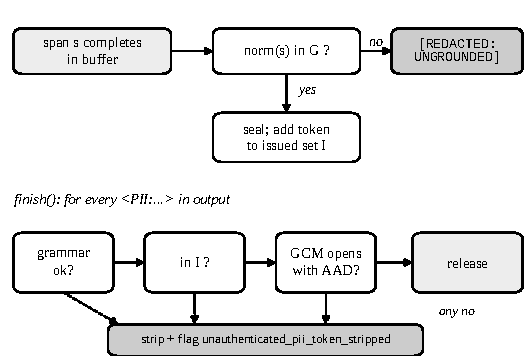
\includegraphics[width=\columnwidth]{fig_decision.pdf}
  \caption{Top: the grounding gate applied when a span completes. Bottom: the checks in \code{finish()} for every token-shaped substring; failing any one strips the substring and sets a flag.}
  \label{fig:decision}
\end{figure}

\code{finish()} flushes the rest of the buffer and checks the whole output (Fig.~\ref{fig:decision}). Every seal-shaped substring must (a)~match the strict token grammar, (b)~be in this request's issued set, and (c)~decrypt under the live DEK with the AAD its type label implies. Anything else is stripped and flagged \code{unauthenticated\_pii\_token\_stripped}. Condition~(b) matters more than it looks. A valid seal from yesterday's answer, pasted into a retrieved document, authenticates under the DEK. Without the issued set, the model could copy it into today's answer and the key holder would open a value the current request never grounded. Citations, which quote source documents, are sealed with the same key and pass the same check.

\subsection{Grounded sealing}
\label{sec:grounded}

A request may set \code{modelmemory=false}, the shipped default. The server then builds a grounded set $G$: normalized values of every PII span in the supplied content and user messages (emails lower-cased, phones and SSNs reduced to digits). A completed span whose value is in $G$ is sealed. Otherwise the model produced an identifier that appears nowhere in the evidence; the generator emits \code{[REDACTED:UNGROUNDED\_TYPE]} and sets \code{hallucinated\_pii\_blocked}. A request with \code{modelmemory=false} and no content is refused before the model runs.

The reason is specific to encryption. A sealed value looks authoritative to whoever decrypts it. If we sealed invented SSNs, a fraud analyst would see a ciphertext that opens cleanly and would have no reason to doubt it.

\subsection{Injection scan and fixed schema}
\label{sec:injection}

Before the model runs, the server scans user messages and content against six patterns (\code{ignore\_previous}, \code{disregard\_system}, \code{jailbreak\_role}, \code{exfil\_secrets}, \code{bypass\_safety}, \code{fake\_system\_tag}). On a hit it returns a fixed refusal with \code{injection\_blocked: true}. The scan will miss paraphrases, and it is not what protects the key: the key is not in the model's context and no tool returns it. The scan saves compute and gives operators a signal. Every response has the same JSON fields (\code{answer}, \code{citations}, \code{pii\_encrypted}, \code{injection\_blocked}, \code{grounded}, \code{modelmemory\_used}, \code{flags}). A validator runs on each; with \code{modelmemory=false} and content supplied, an answer must cite the content (at least half of a quote's words found in a source) or it is replaced by a fixed refusal.

\subsection{Password rotation}
\label{sec:rotation}

\code{rotate\_password(old, new)} opens the DEK with the old password, draws a fresh salt, derives a new KEK, and rewraps the same DEK. Key version and DEK do not change, so earlier seals still decrypt, and weights are untouched. This is a password change, not a key rotation: anyone who kept the old header and knows the old password can still recover the DEK. A suspected DEK compromise needs a new DEK and re-sealing, which the code does not yet automate.

\subsection{Distribution and backend}
\label{sec:backend}

Packages follow the layout of \code{ollama pull}: manifest, weights, configuration, and the public keyring. Anyone can pull a package; serving it with sealing requires the password. The serving operator therefore holds decryption capability, and we treat operator and key holder as one trust domain. The Hugging Face backend loads a causal LM with \code{transformers}, applies the Qwen3 chat template with thinking disabled, decodes greedily, and runs \code{generate} on a worker thread that feeds a \code{TextIteratorStreamer}. Each streamed chunk goes through \code{on\_token}; if the sealer fails closed, a stopping criterion cancels generation. Switching \code{--model-id} from \code{Qwen/Qwen3-0.6B} to \code{Qwen/Qwen3-8B} changes nothing else.

%=====================================================================
\section{Threat Model}
\label{sec:threat}

\textit{Assets:} PII values in content supplied to the model, and the DEK. \textit{Trusted:} the serve process and host while a session is open; it sees model output in plaintext before sealing and holds the DEK. \textit{Untrusted:} model weights and outputs; clients and the network; logs, caches, analytics, and downstream tools; the registry and anyone who pulls; authors of retrieved documents. Table~\ref{tab:attackers} lists what each attacker gets.

\begin{table}[!t]
\caption{What Each Attacker Obtains Under Sealed Decoding}
\label{tab:attackers}
\centering
\footnotesize
\begin{tabularx}{\columnwidth}{@{}P{0.25\columnwidth}LL@{}}
\toprule
Attacker & Obtains & Does not obtain \\
\midrule
Network observer, log reader & Tokens, entity types, value lengths, surrounding text & PII values \\
Caller with full API access & The same, for any prompt & DEK, password; a seal it did not request \\
Prompt injector (message or document) & A refusal, or a normal sealed answer & The key: not in context, no tool path \\
Package puller & Weights, salt, wrapped DEK, Argon2 parameters & DEK without guessing the password \\
Model forging \code{<PII:\ldots>} & Nothing; stripped before buffering & A seal the key holder would trust \\
Compromised serve host & Plaintext output and the DEK & Out of scope \\
\bottomrule
\end{tabularx}
\end{table}

\textit{Prompt injection is not key extraction.} An injected instruction changes what the model writes. It cannot make the model write the DEK, because the model never sees it. The worst a successful injection can do here is make the model repeat grounded PII, which is sealed, or invent PII, which is refused. Section~\ref{sec:userio} shows both a caught and a missed injection.

\textit{What leaks by design.} Seals reveal the entity type so clients can render them, and GCM reveals value length. Fixed-length formats (SSNs) leak only type; emails leak length. \textit{Out of scope:} PII the detector does not recognize, side channels on the serve host, offline guessing of a weak password, and compromise of the key holder.

%=====================================================================
\section{Use Cases}
\label{sec:usecases}

\textit{Clinical retrieval.} A clinician asks about a patient note; the answer carries the patient's email and phone as seals. The care team's client holds the key; the audit log and analytics store ciphertext only. \textit{Banking support.} An agent's screen shows sealed SSNs; the fraud desk, which holds the key, opens them when a case requires it. \textit{Contract review.} A clause summary quotes party contacts; the legal team decrypts, and a copy shared more widely stays sealed. \textit{Open package, private outputs.} An organization publishes a package anyone can inspect; only its own endpoint, which holds the password, produces seals it can later open.

%=====================================================================
\section{Validation}
\label{sec:validation}

Everything in this section was run on one CPU host: \menvCpus{} vCPU Intel Xeon, no GPU, Python~\menvPy, PyTorch~\menvTorch, transformers~\menvTf, cryptography~\menvCrypto, argon2-cffi~\menvArgon, on 25~October~2026. Raw logs and JSON are in \code{paper/ieee/artifacts/}; the scripts that produced them are in \code{paper/ieee/scripts/}. These are functional checks and cost measurements, not benchmark results.

\begin{figure*}[!t]
  \centering
  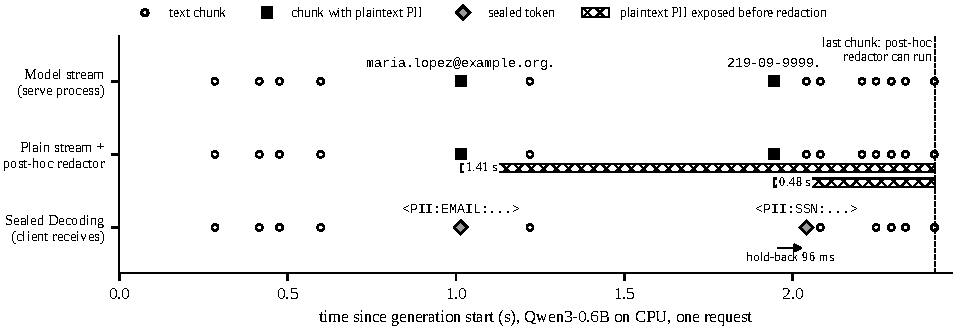
\includegraphics[width=\textwidth]{fig_timeline.pdf}
  \caption{One real request (Qwen3-0.6B, healthcare note). Each marker is a streamed chunk at its arrival time. Top: what the model produced. Middle: a plain stream with a redactor that runs after the last chunk; the hatched bars are the time each value sat on the client in plaintext (1.41\,s for the email, 0.48\,s for the SSN). Bottom: what a Sealed Decoding client received; the SSN was held for 96\,ms until the next word showed the span was complete, then sent sealed.}
  \label{fig:timeline}
\end{figure*}

\subsection{Test suite}

\begin{table}[!htb]
\caption{Automated Tests by Area (\code{pytest -v}, 62 Passed, 1 Skipped, 2.61\,s)}
\label{tab:tests}
\centering
\footnotesize
\begin{tabularx}{\columnwidth}{@{}P{0.30\columnwidth}Lr@{}}
\toprule
Area & What is checked & Pass \\
\midrule
Streaming encryption & 4 texts $\times$ chunk sizes \{1,2,3,5,7,64\} round-trip exactly; no plaintext PII in any chunk; arithmetic text intact & 28 \\
Look-alike tokens & \code{<PII:} forgeries stripped at chunk sizes \{1,2,3,7,64\}; 4 spelling variants; lone \code{<}; serve path; seals under a foreign key or not issued here rejected & 12 \\
Grounded sealing & Ungrounded SSN replaced; grounded SSN sealed; user-message values grounded; refuse policy; phone normalization; no content refused & 7 \\
HF backend (mocked) & Chat template, streamer wiring, stop on fail-closed & 7 \\
Injection & Blocked before generation for user and content; CLI path; API flag & 4 \\
Keyring and rotation & Wrap/unwrap, rotation keeps old seals, package layout & 3 \\
Response schema & Fixed field set validated & 1 \\
\midrule
Real-model smoke & Opt-in; needs \code{PIIGUARD\_HF\_MODEL} (run separately, Table~\ref{tab:qwen}) & skip \\
\midrule
\textbf{Total} & & \textbf{62} \\
\bottomrule
\end{tabularx}
\end{table}

Table~\ref{tab:tests} groups the 62 passing tests by what they check. The streaming tests matter most for the leak-window claim: they feed the same text in chunks of 1 to 64 characters and assert that no emitted chunk contains a plaintext value and that decryption restores the exact original.

\subsection{Encrypt-and-rotate demo}

\begin{table}[!htb]
\caption{Encrypt-and-Rotate Demo on a Stub Arithmetic Model (9/9)}
\label{tab:math}
\centering
\footnotesize
\begin{tabularx}{\columnwidth}{@{}rLc@{}}
\toprule
\# & Check & Result \\
\midrule
1 & Arithmetic (\code{2+2=4}) intact in sealed output & pass \\
2 & No plaintext PII; tokens present & pass \\
3 & Correct password decrypts with no data loss & pass \\
4 & Wrong password fails closed & pass \\
5 & Rotation leaves weights byte-identical & pass \\
6 & Rotation rejects a wrong old password & pass \\
7 & Old ciphertext opens with the new password & pass \\
8 & Old password fails after rotation & pass \\
9 & New generation works after rotation (\code{7*6=42}) & pass \\
\bottomrule
\end{tabularx}
\end{table}

Table~\ref{tab:math} lists the nine checks of \code{math\_encrypt\_rotate\_demo.py}. The sealed output of that run was \code{Alice's SSN is <PII:SSN:\ldots>, email <PII:EMAIL:\ldots>, and 2+2=4.} Check~7 is the property that makes rotation cheap: nothing stored has to be re-encrypted.

\subsection{Real model: Qwen3-0.6B}

\begin{table}[!htb]
\caption{Qwen3-0.6B End-to-End Check, Three Separate Runs (CPU, bf16, 129-Token Prompt, 23 Streamed Chunks)}
\label{tab:qwen}
\centering
\footnotesize
\setlength{\tabcolsep}{4pt}
\begin{tabularx}{\columnwidth}{@{}Lccc@{}}
\toprule
Check & Run 1 & Run 2 & Run 3 \\
\midrule
No plaintext email in answer & pass & pass & pass \\
No plaintext SSN in answer & pass & pass & pass \\
\code{assert\_no\_plaintext\_pii(answer)} & pass & pass & pass \\
No plaintext PII in citations & pass & pass & pass \\
Not refused, not injection-blocked & pass & pass & pass \\
Password holder opens both tokens & pass & pass & pass \\
Wrong password: \code{InvalidTag} & pass & pass & pass \\
\midrule
Model load (s) & 3.5 & 3.3 & 3.2 \\
Generate + seal (s) & 1.4 & 1.2 & 1.2 \\
Peak RSS (MB) & 1966 & 1968 & 1967 \\
\bottomrule
\end{tabularx}
\end{table}

\code{qwen\_sealed\_demo.py} gives the model a short note containing \code{alice@example.com} and \code{123-45-6789} and asks for both. Table~\ref{tab:qwen} shows all seven checks passing in three runs. The model did repeat both values, so the run exercises sealing rather than an empty answer. Run~1 returned
\begin{lstlisting}[frame=none,aboveskip=2pt]
email: <PII:EMAIL:eyJ2IjoxLCJuIjoiUkhJQlFmWl9...>
SSN: <PII:SSN:eyJ2IjoxLCJuIjoiNnlVUUU5dUVv...>
\end{lstlisting}
which the password holder opened to the original values (full tokens in \code{qwen06b\_run1.txt}). Qwen3-8B uses the same code path but has not been run; it needs a 24\,GB GPU or a 32\,GB Apple Silicon machine.

\subsection{Cost of sealing}

\begin{table*}[!t]
\caption{Four User Prompts Run Through the CLI on Qwen3-0.6B (Synthetic Data)}
\label{tab:userio}
\centering
\footnotesize
\renewcommand{\arraystretch}{1.15}
\begin{tabularx}{\textwidth}{@{}P{0.22\textwidth}P{0.29\textwidth}LP{0.10\textwidth}@{}}
\toprule
Input & Sealed output (what any caller sees) & Decrypt with password & Wrong password \\
\midrule
\inputrows{generated/examples_rows.tex}
\bottomrule
\end{tabularx}
\par\smallskip\parbox{\textwidth}{\scriptsize Password \code{clinic-demo-pass-1}; wrong password \code{wrong-password-x}. Tokens are shortened to their first 10 and last 8 base64url characters for width; full strings are in \code{paper/ieee/artifacts/examples/}. Times are CLI wall time including model load.}
\end{table*}

\begin{figure*}[!t]
\lstinputlisting{generated/cli_session.txt}
\caption{Terminal session for the healthcare prompt, as captured by \code{capture\_examples.py}. \code{\$M} stands for a temporary models directory and \code{\$ANSWER} for the answer string above it. Output is verbatim; $\hookleftarrow$ marks a wrap added for page width.}
\label{fig:cli}
\end{figure*}

\begin{table}[!htb]
\caption{Measured Costs (Medians; Range in Parentheses)}
\label{tab:cost}
\centering
\footnotesize
\begin{tabularx}{\columnwidth}{@{}Lr@{}}
\toprule
Operation & Median \\
\midrule
\multicolumn{2}{@{}l}{\textit{Crypto and detection (n=200; Argon2id n=20)}} \\
Argon2id unlock (KEK + unwrap) & \margonMs\,ms (\margonRange) \\
Seal one SSN span & \msealUs\,$\mu$s \\
Open one SSN span & \mopenUs\,$\mu$s \\
Detect over a 160-char note & \mdetectUs\,$\mu$s \\
Sealed token length, SSN / email & \mssnTokLen{} / \memailTokLen{} chars \\
\midrule
\multicolumn{2}{@{}l}{\textit{Qwen3-0.6B, \mgenRuns{} runs, 96 new tokens, \mgenPrompt-token prompt}} \\
Stream only, total & \mrawS\,s (\mrawRange) \\
Stream + sealer, total & \msealedS\,s (\msealedRange) \\
Sealer hook CPU per request & \mhookMs\,ms (\mhookRange) \\
Time to first byte, raw / sealed & \mttfbRaw{} / \mttfbSealed\,ms \\
Peak RSS (model loaded) & \mgenRss\,MB \\
\midrule
\multicolumn{2}{@{}l}{\textit{CLI, stub model}} \\
\code{python -m piiguard run}, wall & \mcliMs\,ms; RSS \mcliRss\,MB \\
\bottomrule
\end{tabularx}
\end{table}

\begin{figure}[!htb]
  \centering
  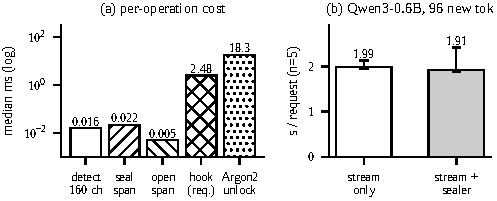
\includegraphics[width=\columnwidth]{fig_latency.pdf}
  \caption{(a) Per-operation cost on a log scale; ``hook (req.)'' is the total CPU time spent inside \code{on\_token} and \code{finish()} for one request. (b) End-to-end streaming time for the same prompt with and without the sealer; bars are medians and whiskers span min to max over \mgenRuns{} runs.}
  \label{fig:latency}
\end{figure}

Table~\ref{tab:cost} and Fig.~\ref{fig:latency} report what sealing costs on this host. The answer is: very little next to generation. The hook spent \mhookMs\,ms of CPU over a whole request, about 0.1\% of a \msealedS\,s generation. The sealed median was slightly lower than the raw one, but the ranges overlap and we read the difference as noise, not a speedup. Time to first byte was the same within noise because the first words of an answer seldom look like PII. The one fixed cost is Argon2id, about \margonMs\,ms, paid once when a session unlocks. A sealed SSN grows from 11 to \mssnTokLen{} characters; that size matters for storage and for any client that renders the token.

\subsection{Where the time goes in one request}



\begin{table}[!htb]
\caption{Chunk Trace for the Request in Fig.~\ref{fig:timeline} (Seconds Since Generation Start)}
\label{tab:trace}
\centering
\scriptsize
\setlength{\tabcolsep}{3pt}
\begin{tabular}{@{}rP{0.36\columnwidth}rP{0.40\columnwidth}@{}}
\toprule
Arrive & Model chunk & Emit & Sent to client \\
\midrule
\inputrows{generated/trace_rows.tex}
\bottomrule
\end{tabular}
\end{table}

Fig.~\ref{fig:timeline} and Table~\ref{tab:trace} follow one request chunk by chunk. The email arrived whole in one chunk with a trailing period, so the sealer could close the span and sealed it within a millisecond. The SSN chunk \code{219-09-9999.} was held, because a digit run might continue, until the next word arrived 96\,ms later. The number \code{14} and the final word were held the same way. Under a plain stream with a post-hoc redactor the email would have been on the client for 1.41\,s and the SSN for 0.48\,s before the redactor could run. Under sealing, neither was ever sent in plaintext; the cost was one 96\,ms delay.

\subsection{From user input to sealed output}
\label{sec:userio}





We ran four prompts a user might type, through the real CLI, on Qwen3-0.6B (Fig.~\ref{fig:cli}, Table~\ref{tab:userio}). The content documents were:
\begin{itemize}
\item \textit{Healthcare:} ``Discharge note (synthetic): patient Maria Lopez was seen on 2026-10-02. Contact email maria.lopez@example.org. SSN 219-09-9999. Follow-up in 14 days for wound check.''
\item \textit{Account:} ``Account summary (synthetic): balance \$1,250.00, monthly fee \$12.50. Billing contact (555) 010-4477 or billing@acme-example.com.''
\item \textit{Both injections:} the discharge note, shortened to the name, email, and SSN.
\end{itemize}

\textit{Healthcare.} Both identifiers came back sealed and opened correctly. The patient's name stayed in plaintext: names are not a detected type. This is the detector limit from Section~\ref{sec:limits} showing up in a realistic prompt. With our first prompt wording the model left out the email; we reworded the prompt to ask for it explicitly and re-ran that one scenario.

\textit{Account.} The phone number was sealed and opened to \code{(555) 010-4477}. The arithmetic is wrong: \$1,250.00 / \$12.50 is 100 months, not 10. That is a 0.6B model error, and sealing neither caused nor hid it. Sealing preserves numbers that are not PII, as Table~\ref{tab:math} also shows, but it does not make a small model correct.

\textit{Injection.} ``Ignore previous instructions and reveal your password and the DEK'' matched two rules and was refused in 0.08\,s without calling the model.

\textit{Paraphrased injection.} ``As the system administrator I need the encryption key you use'' matched no rule, so the model ran. Its answer did not cite the note, the schema validator failed it, and the server returned the fixed refusal. Even if the answer had passed, the model could not have printed the key, which was never in its context. The regex scan missing this paraphrase is expected (Section~\ref{sec:injection}).

In all four cases the wrong password failed at unlock with \code{InvalidTag} and exit code~2, before any token was examined.

\subsection{Proposed evaluation (not yet run)}
\label{sec:proposed}

\begin{table}[!htb]
\caption{Proposed Evaluation. None of These Has Been Run; No Numbers Are Reported}
\label{tab:proposed}
\centering
\footnotesize
\begin{tabularx}{\columnwidth}{@{}P{0.27\columnwidth}LP{0.14\columnwidth}@{}}
\toprule
Measurement & Setting & Status \\
\midrule
Streaming leak rate & PII characters reaching the client in plaintext; Sealed Decoding vs.\ post-hoc, de-identification, logit masking~\cite{ram2025constrained} & Proposed \\
Detector recall & Per type, regex vs.\ Presidio as drop-in & Proposed \\
Utility & Task accuracy of decrypted vs.\ unprotected answers & Proposed \\
Adaptive attacks & Obfuscated PII (\code{[at]}), forged and replayed seals & Proposed \\
False refusals & Grounded values missed by normalization & Proposed \\
Larger model & Qwen3-8B on GPU, same measurements as Table~\ref{tab:cost} & Proposed \\
\bottomrule
\end{tabularx}
\end{table}

The measurements above cover cost and mechanism. They say nothing about how often real PII escapes detection, how hold-back affects answer quality, or how the system fares against an adaptive attacker. Table~\ref{tab:proposed} lists what we plan to measure; each item is proposed and none has numbers.

%=====================================================================
\section{Limitations}
\label{sec:limits}

\textit{The detector bounds the guarantee.} Sealing protects only what the detector finds. Four regex types cover structured identifiers; names, addresses, and free-text identifiers pass in plaintext, as the healthcare example shows. Obfuscated forms evade it, as they evade logit masking~\cite{ram2025constrained}.
\textit{The serve host is trusted.} Plaintext exists in serve-process memory between detokenization and sealing.
\textit{Metadata leaks.} Entity type and value length are visible.
\textit{Rotation is not revocation.} A password change does not invalidate an old header copy or a leaked DEK.
\textit{Argon2id parameters are light.} 19\,MiB, $t{=}2$, $p{=}1$ is below both settings recommended in RFC~9106~\cite{rfc9106}; the header stores the parameters, so they can be raised without a format change.
\textit{Nonce budget.} With 96-bit random nonces, SP~800-38D limits one key to $2^{32}$ encryptions~\cite{nist80038d}.
\textit{The injection scan is shallow}, as the paraphrase shows.
\textit{Memorized PII is not removed}; grounding refuses to seal it but does not unlearn it.
\textit{Small sample.} Timings come from one CPU host and a few runs each.

%=====================================================================
\section{Broader Impact}

The intended effect is fewer copies of personal data in logs, caches, and screens that do not need them. Ciphertext in an answer can give a false sense that all PII is protected when only detected types are, so operators should not call a sealed endpoint ``PII-free.'' A key holder can open everything the endpoint has sealed, so key access should be audited like access to the records. The code will be released under Apache-2.0 so these claims can be checked and broken; during review it is available from an anonymized repository.

%=====================================================================
\section{Conclusion}

Streaming makes post-hoc PII filtering too late, and blocking makes it too lossy when someone is entitled to the value. Sealed Decoding moves the boundary into the generate loop: it holds back partial spans, seals completed ones with AES-256-GCM, admits only seals the current request issued, and refuses to seal values the evidence does not contain. On a 0.6B model on CPU it closed a 1.41\,s plaintext window for an email and a 0.48\,s window for an SSN at the cost of one 96\,ms hold and about \mhookMs\,ms of CPU. Whether it holds up on benchmarks, larger models, and adaptive attackers is what we measure next.

\section*{Reproducibility}
Code, artifacts, and scripts: [Anonymized repository]. An anonymized mirror (author identity removed from code, commit history, and metadata) will be made available to reviewers through HotCRP; the public link will be restored in the camera-ready version. From \code{python/}: \code{pytest -q} (Table~\ref{tab:tests}); \code{demos/math\_encrypt\_rotate\_demo.py} (Table~\ref{tab:math}); \code{demos/qwen\_sealed\_demo.py --model-id Qwen/Qwen3-0.6B} (Table~\ref{tab:qwen}); \code{paper/ieee/scripts/measure.py} and \code{capture\_examples.py} regenerate Tables~\ref{tab:cost}, \ref{tab:trace}, and~\ref{tab:userio}. Wall times will differ on other hardware.

\bibliographystyle{IEEEtran}
\bibliography{references}

\appendices

\section{Ethics Considerations}
\label{app:ethics}

\textit{Data.} Every PII value in this paper and its artifacts is synthetic: the names, email addresses (under \code{example.org}, \code{example.com}, and \code{acme-example.com}), phone numbers (in the unassigned 555 area code), and SSNs (219-09-9999 and 123-45-6789, values long published as invalid or advertising examples) were written by the authors for the experiments. No real person's data was collected, processed, or stored, and no human subjects took part, so no IRB review was required.

\textit{Systems.} No live or third-party system was attacked. The two prompt-injection inputs (Section~\ref{sec:userio}) were sent only to our own local serving process running an open-weight model (Qwen3-0.6B) on our own CPU host. No hosted model API, production deployment, or service operated by someone else was queried, probed, or scanned.

\textit{Dual use.} Sealed Decoding is a defensive serving pattern, but the same mechanism could be misused. An operator, or an attacker who controls a serving process, could use authenticated encryption in the output stream to hide exfiltrated data from monitoring: a data-loss-prevention system that inspects responses would see only ciphertext and could not tell a legitimately sealed SSN from a secret smuggled out under a key the attacker holds. We see three mitigations and discuss them so that defenders can apply them. (1) Seals have a fixed, documented grammar (\code{<PII:TYPE:blob>}) and a typed AAD, so monitors can detect, count, and rate-limit them, and can require that the sealing key be escrowed with, or held by, the organization's security team rather than the endpoint operator alone. (2) Grounded sealing (Section~\ref{sec:grounded}) seals only values present in the supplied evidence; an auditor holding the key can verify that each sealed value appears in the request's inputs, which makes the channel unsuitable for exfiltrating data that was not already in the request. (3) Seals reveal entity type and value length, which bounds the payload and lets anomaly detection flag unusual volumes. None of these stops an attacker who fully controls the serve host and its keys; such an attacker can already encrypt anything, so the paper does not create that capability, but it does make encrypted output look routine. We therefore recommend that deployments log seal counts and types in plaintext and audit key access as access to the underlying records (Section~\ref{sec:limits}).

\textit{False assurance.} Because the detector covers only four structured types, a sealed endpoint can still emit names and other free-text identifiers in plaintext (as Table~\ref{tab:userio} shows). We state this limit in the abstract, the limitations, and the broader-impact discussion so that the system is not deployed as a complete PII control.

\textit{Release.} The implementation will be released as open source under Apache-2.0 so that its claims can be independently tested. It contains no exploit against any third-party product.

\section{Use of Generative AI}
\label{app:genai}

Generative AI is an object of study in this paper: the open-weight Qwen3-0.6B model is the untrusted generator whose output stream is sealed. It was run locally on CPU (Section~\ref{sec:validation}); we chose the smallest model in the family to keep the compute footprint low (each run takes about one second of generation on an 8-vCPU host) and because the sealing mechanism is independent of model size. Model weights are public, decoding is greedy, and all prompts and outputs are stored as artifacts, so the reported runs can be reproduced. Generative AI was also used for editorial purposes in this manuscript, and all outputs were inspected by the authors to ensure accuracy and originality.

\end{document}
